\chapter{Application and validation}

\begin{comment}
name should be changed, what we actually done to validate the platform
or just virtual platform
in order to validate and improve the performance of temperature estimation algorithm, several 
models is imported.

here we talk about what model is used to generate raw data for validation
\end{comment}


After the theoretical basis of the virtual experiment platform is known and 
the program of the virtual experiment platform is built, the application should be 
verified with experiment data generated based on the real experiment.

\begin{figure}[htbp]
    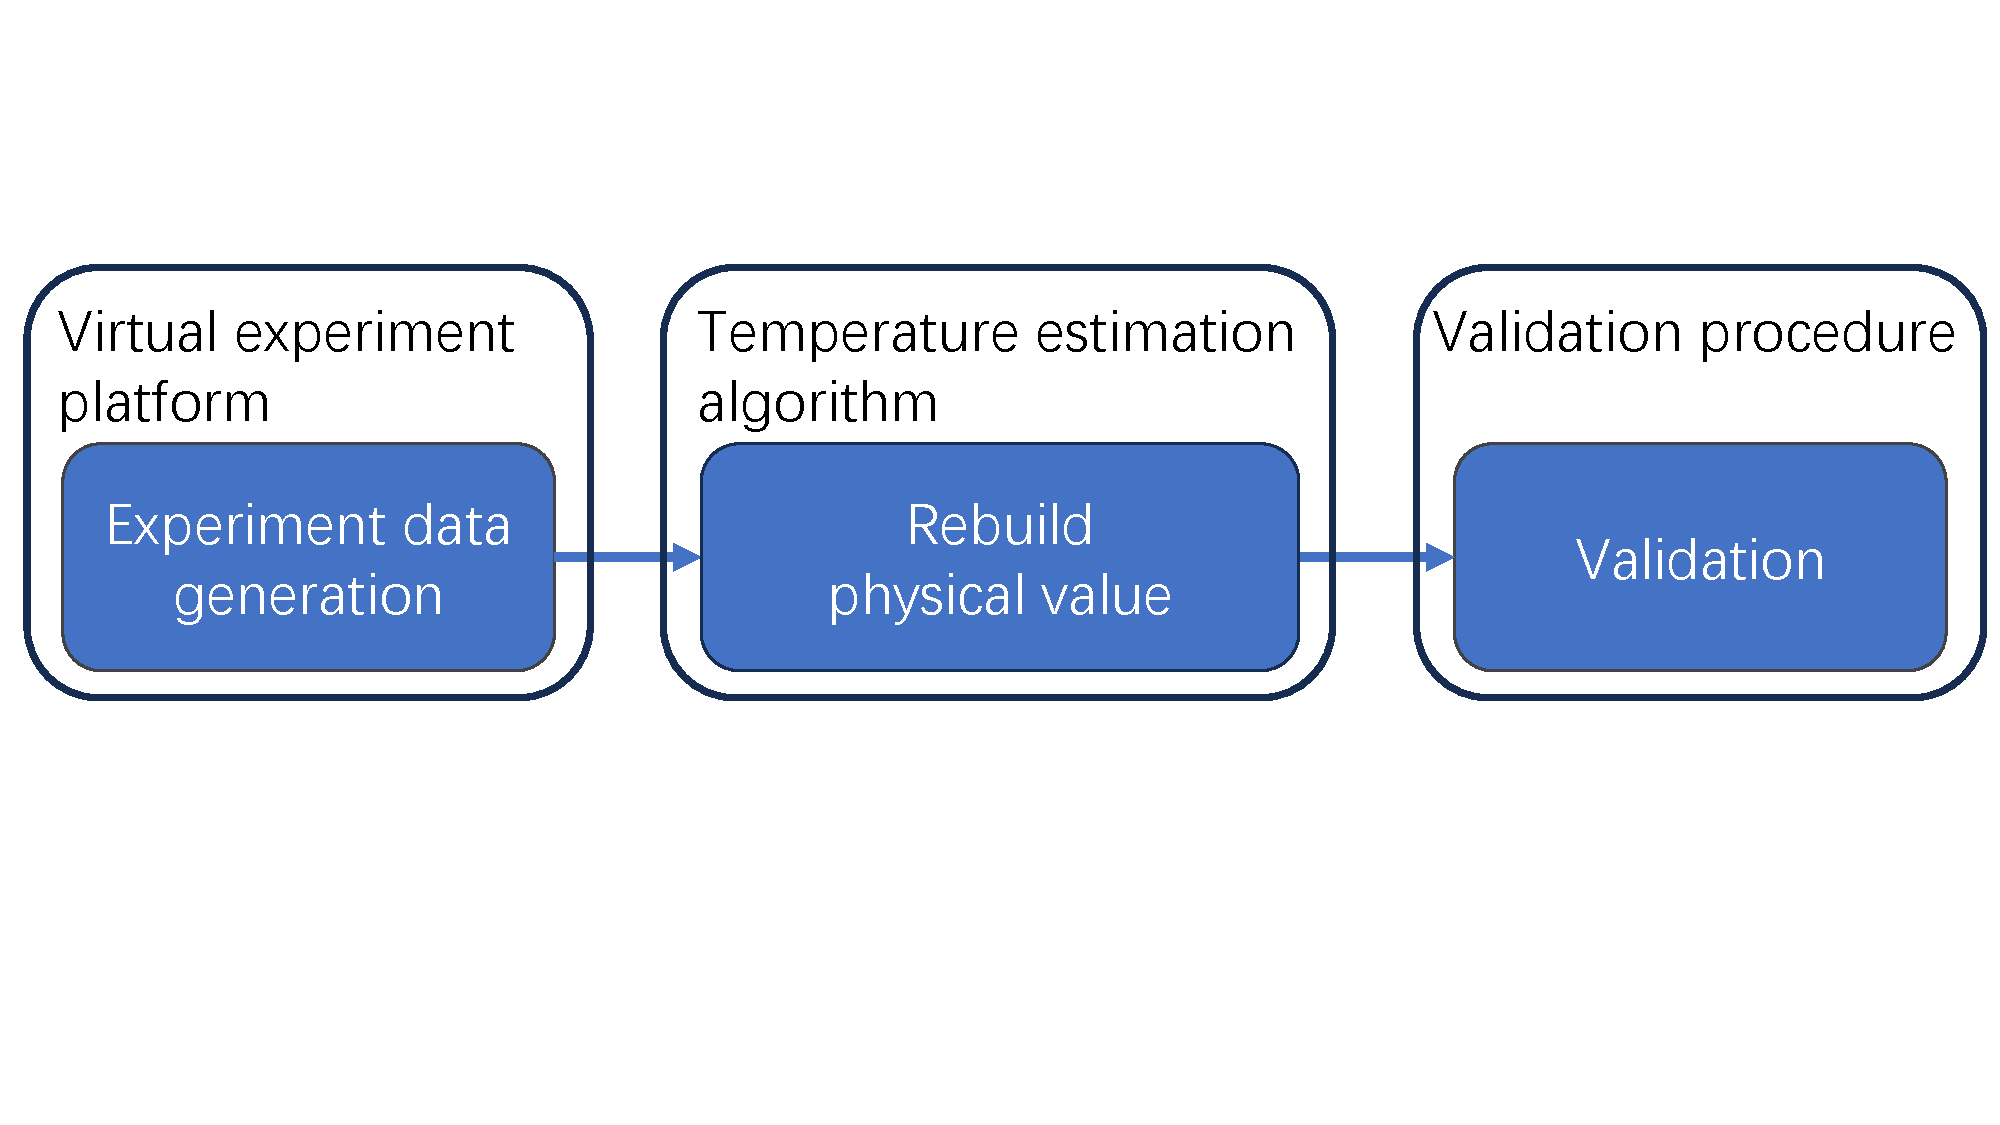
\includegraphics[width=0.95\textwidth]{figures/application_procedure.pdf}
    \caption{Complete procedure from data generation to model validation}
    \label{fig: application_procedure}
\end{figure}

\section{Experiment data generation}
\subsection{Temperature field}%
\subsection{Emissivity model}%
\subsection{Integration method}
\section{Rebuild Physical value}
\subsection{Emissivity model used for calculation}

\subsection{Curve fit algorithm}

\subsection{Parameters in calculation}
quantum efficiency, lens factor

\section{Validation}